\chapter{Ciclo de Vida do Sistema}
\section{Definição da Abordagem}
Como a parte inicial do projeto, com um período de aproximadamente 6 meses, seria realizada pelo próprio autor, a disponibilidade do cliente ser mais abrangente, o projeto for evoluido conforme o tempo e novas necessidades forem surgindo, definiu-se a utilização de uma abordagem de desenvolvimento ágil \cite{beck2001agile}. A metodologia definida foi o \textit{Extreme Programming} \cite{beck_2004}, visando sempre estar evoluindo o sistema com \textit{feedbacks} do cliente, produzindo código com padrões de codificação e simples para possíveis manuntenções no futuro.

Para auxiliar nas \textit{releases} do projeto, utilizou-se o conceito de \textit{sprints}, provinda do \textit{Scrum} \cite{scrum_guide}. O Scrum é um framework estrutural flexível utilizado para gerenciar o desenvolvimento de produtos complexos empregando, com o auxílio de sprints, uma abordagem iterativa e incremental para aperfeiçoar a previsibilidade e o controle de riscos. As \textit{sprints} são pequenos intervalos de tempo, de um mês ou menos, durante o qual uma versão incremental potencialmente utilizável do produto é criada. Uma nova Sprint inicia imediatamente após a conclusão da Sprint anterior.

\section{Contexto e Necessidades}
Tendo como problema a falta de monitoramento energético adequado na Universidade de Brasília, foi realizado um estudo sobre o contexto para identificar as necessidades do cliente. Tal estudo abordava o entendimento de fatores energéticos cruciais, como por exemplo sistemas trifásicos, horários de ponta e fora de ponta, tensão, corrente, resistência e afins.

Com um entendimento melhor do contexto, algumas reuniões foram feitas com o cliente e foram obtidas as seguintes necessidades:

\begin{itemize}
    \item Cada campus da Universidade de Brasília deve ser responsável por realizar seu próprio monitoramento energético.
    \item O campus Darcy Ribeiro deve funcionar como uma espécie de administração central.
    \item As medições devem ser registradas de maneira adequada e poderão ser resgatadas, conforme um período de tempo especificado.
\end{itemize}

Um dos pontos levantados nas reuniões foi o de um possível monitoramento, no futuro, de medições de água. Tendo em vista esses recursos que seriam monitorados e de possíveis outros, definiu-se o nome do projeto como Sistema de Monitoramento de Insumos - Universidade de Brasília (SMI-UnB). Definiu-se, também, que para o contexto inicial seriam enfatizados os dados de energia e que seriam entregues duas \textit{releases}, de aproximadamente 80 dias, sendo essas:

\begin{itemize}
    \item Release 1: coleta dos dados de energia.
    \item Release 2: apresentação dos dados e comunicação inter-campi.
\end{itemize}

Deginiu-se que a hospedagem do código/documentação do projeto e o controle de mudanças seriam realizados utilizando-se o \textit{software} livre GitLab CE\footnote{\url{https://gitlab.com/gitlab-org/gitlab-ce}} e para controlamento de versão, a ferramenta Git\footnote{\url{https://git-scm.com/}}.

A escolha do GitLab CE se deve pela cultura de \textit{software} livre, pois o projeto teria um âmbito acadêmico, o compartilhamento de conhecimento poderia ser realizado de maneira mais fácil e a qualidade final não seria comprometida \cite{raymond1999}.

A licença escolhida para o projeto foi a MIT. Ela consiste em uma licença permissiva, autorizando o uso comercial, modificação, distribuição e sublicenciamento \cite{mit_license}.

\section{Requisitos}
Com as necessidades em mãos e o repositório do projeto criado, utilizou-se o propósito das estórias de usuário \cite{beck_2004}, de uma maneira mais simplificada, em \textit{milestones} no repositório, as quais possuiriam diversas \textit{issues} e essas \textit{issues} apresentariam uma terminologia mais técnica da solução em si. Uma \textit{milestone} pode possuir uma data início/fim e é composta por um aglomerado de problemas, comumente chamados de \textit{issues} \cite{gitlab}.

Vale ressaltar que as \textit{milestones} e \textit{issues} foram criadas acompanhando o decorrer do projeto, ou seja, a cada \textit{sprint}, era avaliado se ocorreram mudanças de escopo, quais seriam as \textit{issues} da próxima \textit{sprint}, se era necessário criar uma nova \textit{milestone} etc.

\section{Tecnologias Escolhidas}
Buscando atender toda a conectividade esperada pelo projeto e trazer benefícios ao cliente, definiu-se que sistema teria uma implementação \textit{web}. Sistemas \textit{web} não necessitam de instalação por parte do usuário final, facilitando bastante o processo de implantação e podem ser acessados a partir de qualquer lugar e em qualquer plataforma \cite{pressman_2009}.

Definiu-se utilizar o \textit{framework} \textit{web} Django, por o mesmo realizar facilmente a integralização, desde a comunicação com o banco de dados até a apresentação de dados para o usuário final. Além disso, o banco de dados escolhido foi PostgreSQL, que assim como o Django, também trata-se de um \textit{software} livre.

    \subsection{Django}

    O Django \cite{django_project} é um \textit{framework} para desenvolvimento \textit{web} implementado na linguagem Python\footnote{\url{https://www.python.org/}}. Sua arquitetura inspira-se no modelo tradicional MVC(\textit{Model} \textit{View} \textit{Controller}), porém, com algumas especificidades. A comunidade \textit{Django} adota o acrônimo MTV (\textit{Model} \textit{Template} \textit{View}), onde os papéis de \textit{model}, \textit{view} e \textit{controller} são redefinidos como:
    \begin{itemize}
        \item \textit{Model}: corresponde à \textit{model} do MVC tradicional e representa as classes que popularão as tabelas do banco de dados. O \textit{Django} possui um ORM (\textit{Object-Relational Mapping}, Mapeamento de Objeto Relacional) para realizar a manipulação dessas tabelas, não sendo necessário a escrita de consultas em SQL para a persistência das informações.
        \item \textit{Template}: corresponde aproximadamente à \textit{view} do MVC tradicional e descreve como as informações serão apresentadas para o usuário.
        \item \textit{View}: representada por uma função \textit{callback} referente à uma classe de URLs, descrevendo quais informações serão apresentadas e como elas serão enviadas para o \textit{template}. Alguns autores defendem que a view corresponde ao \textit{controller} do MVC tradicional, mas os próprios desenvolvedores do \textit{Django} a \textit{view} deve ser minimalista e boa parte do papel do \textit{controller} deve ser implementado nas próprias classes dos modelos.
    \end{itemize}

    Na nomenclatura do \textit{Django}, um conjunto de funcionalidades pode ser agrupado em aplicação. Cada aplicação possui suas próprias \textit{models}, \textit{views} e \textit{templates}.

    A Figura \ref{django-arq} mostra a arquitetura do \textit{Django}, apresentando as camadas do MTV durante a comunicação com o navegador até o acesso ao banco de dados. O \textit{URL dispatcher} identifica endereços requisitados pelo usuário e realiza o redirecionamento da requisição para a aplicação correta. A coordenação de requisições entre o \textit{URL dispatcher} e a \textit{view} e da \textit{view} até o \textit{template} é feita pelos chamados \textit{Middlewares}. Os \textit{Middlewares} realizam a persistência de informações entre as diferentes camadas.

    \begin{figure}[h]
        \centering
        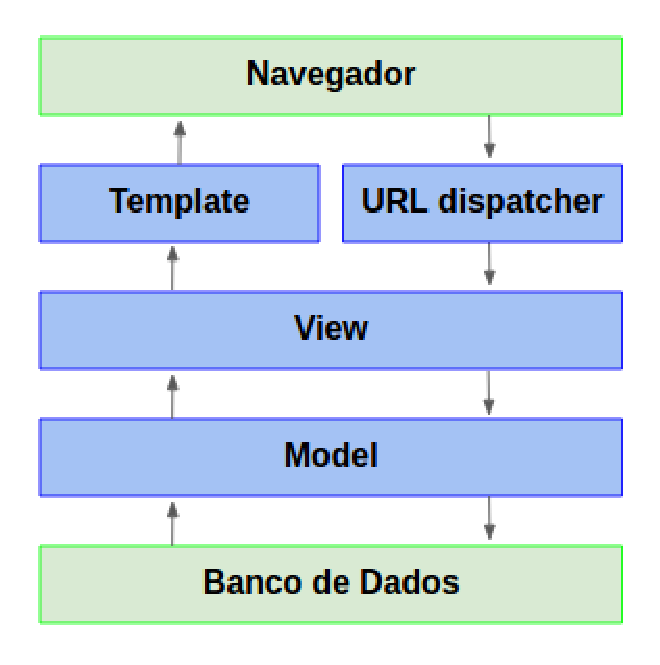
\includegraphics[keepaspectratio=true,scale=0.5]{figuras/django-arquitetura.eps}
        \caption{Arquitetura MTV \textit{Django}}
        \label{django-arq}
    \end{figure}

\section{Protocolos Utilizados}
Antes de começar o desenvolvimento, foi necessário realizar um profundo estudo sobre o equipamento para medição de dados de energia, comumente chamado de transdutor, visto que esse já havia sido pré-designado para utilização, devido a contratos realizados anteriormente pela Universidade de Brasília.

O equipamento em questão foi o TR 4020, Figura \ref{tr4020}, disponibilizado pela empresa Embrasul\footnote{\url{http://www.embrasul.com.br/}}. Segundo seu manual, possui frequência de amostragem a cada 50ms, comunica-se utilizando o protocolo de comunicação Modbus, no modo RTU com velocidade de 10M/100Mbps em sistemas Ethernet utilizando o protocolo UDP como transporte. No datagrama UDP, no campo de dados, o protocolo ModBUs - RTU é encapsulado, sendo que a porta de comunicação padrão é a 1001. O endereço ModBus dos equipamentos por padrão é 1, onde a diferenciação entre equipamentos se dá pelo número de IP.

\begin{figure}[h]
    \centering
    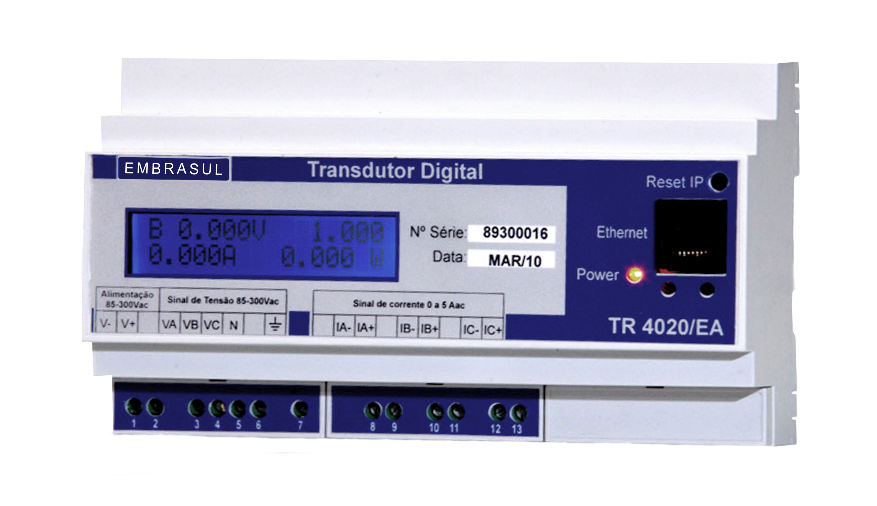
\includegraphics[keepaspectratio=true,scale=0.5]{figuras/tr4020.eps}
    \caption{Transdutor TR4020}
    \label{tr4020}
\end{figure}

    \subsection{\textit{Modbus RTU}}

    \textit{Modbus} é um protocolo serial utilizado para transmitir informações entre dispositivos eletrônicos. Suas mensagens utilizam a arquitetura de mestre-escravo, como mostrado na figura \ref{mestre_escravo} \cite{modbus}. Nesta arquitetura, o papél de mestre é designado ao dispositivo que envia as requisições e escravo ao que responde passivamente às mesmas.

    \begin{figure}[!htpb]
        \centering
        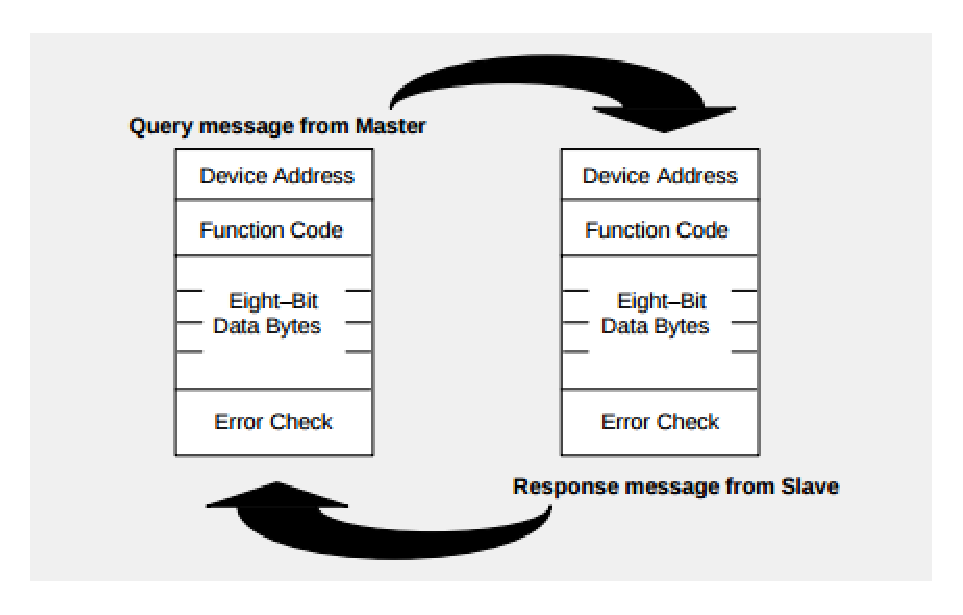
\includegraphics[keepaspectratio=true,scale=0.8]{figuras/mestre_escravo.eps}
        \caption{Comunicação Mestre-Escravo \textit{Modbus}. Fonte: \cite{modbus}}
        \label{mestre_escravo}
    \end{figure}

    Quando controladores são configurados para se comunicarem em uma rede Modbus usando o modo RTU (\textit{Remote Terminal Unit}, Unidade de Terminal Remoto) cada \textit{byte} contém duplas hexadecimais de 4 \textit{bits}. A maior vantagem de utilizar este modo é que sua grande densidade de caracteres permite uma maior taxa de transferência comparado ao modo ASCII em uma mesma taxa de transmissão \cite{modbus}.

    Uma mensagem em Modbus RTU possui 16 \textit{bytes} e é definida da seguinte maneira:
    \begin{itemize}
        \item Identificador do Aparelho: 2 \textit{bytes}.
        \item Código de Função: 2 \textit{bytes}, define qual tipo de operação o equipamento irá realizar.
        \item Campo de Dados: 8 \textit{bytes}, sendo 4 \textit{bytes} para indicar o endereço do primeiro registrador requisitado e 4 \textit{bytes} para indicar a quantidade de registradores que serão lidos.
        \item CRC (\textit{Cyclic Redundancy Check}, Verificação de Redundância Cíclica): 4 \textit{bytes} para verificação de erros.
    \end{itemize}

    A resposta do escravo possui a seguinte estrutura:

    \begin{itemize}
        \item Identificador do Aparelho: 2 \textit{bytes}.
        \item Código de Função: 2 \textit{bytes}, define qual tipo de operação o equipamento irá realizar.
        \item Tamanho do{payload}: 2 \textit{bytes}, define o tamanho do campo de dados em \textit{bytes}.
        \item Campo de dados: possui tamanho variável, de acordo com o valor do campo anterior.
        \item CRC (\textit{Cyclic Redundancy Check}, Verificação de Redundância Cíclica): 4 \textit{bytes} para verificação de erros.
    \end{itemize}

    \subsection{UDP}
    A camada de transporte é...

    Ethernet é...

    IP é...

    O protocolo UDP (\textit{User Datagram Protocol}, Protocolo de Datagrama do Usuário) é um protocolo da camada de transporte e não orientado a conexões. Seu cabeçalho, figura \ref{udp_header}, possui 8 \textit{bytes}, seguido de uma carga útil. As portas apresentadas no cabeçalho representam as máquinas de origem e destino \cite{tanenbaum_2002}.

    \begin{figure}[!htpb]
        \centering
        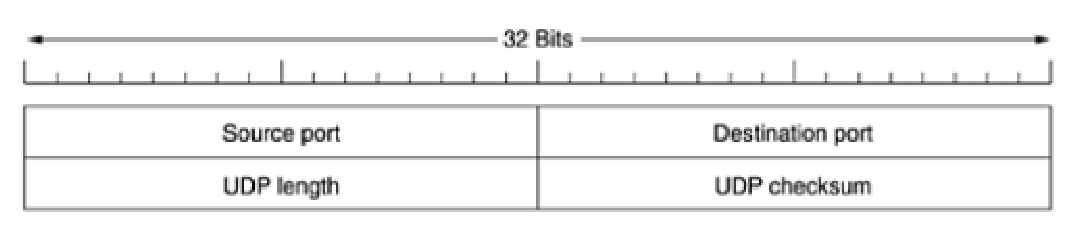
\includegraphics[keepaspectratio=true,scale=0.8]{figuras/udp_header.eps}
        \caption{Cabeçalho do UDP. Fonte: \cite{tanenbaum_2002}}
        \label{udp_header}
    \end{figure}

\section{Desenvolvimento}
O processo de desenvolvimento teve início dia 08/08/2016 e fim 23/06/2017, conforme o cronograma ilustrado nas figuras X Y e Z.
